\documentclass[12pt,fleqn]{beamer}


\xdefinecolor{lavendar}{rgb}{0.8,0.6,1}
\xdefinecolor{olive}{cmyk}{0.64,0,0.95,0.4}
%\xdefinecolor{olive}{cmyk}{1,0,0,0}
\xdefinecolor{mag}{cmyk}{0.1,1,0,0.2}
\xdefinecolor{lblue}{rgb}{0,0,1.5}
\xdefinecolor{lred}{rgb}{1,0,0}
\xdefinecolor{mine}{cmyk}{1,0,0.2,0}
\xdefinecolor{bluel}{cmyk}{0.1,0,0.9,0.4}

\usepackage{amsmath,amssymb,dsfont,mathrsfs}
\usepackage{tikz,pgflibraryplotmarks}
\usepackage{multimedia}
\usepackage{wasysym}
\usepackage{rotating}
\usepackage{algorithm,algorithmic}
\usepackage{graphicx} % more modern
\usepackage{subfigure}
\usepackage{booktabs}

\usepackage{pgfplots}
\usepackage{verbatim}

\usepackage{setspace}
\newlength\iwidth
\newlength\iheight

\newcommand\makebeamertitle{\frame{\maketitle}}%
\graphicspath{{./images/}}
\setbeamertemplate{navigation symbols}{}
\addtobeamertemplate{navigation symbols}{}{%
    \usebeamerfont{footline}%
    \usebeamercolor[fg]{footline}%
	\insertshorttitle
    \;--
    \insertframenumber
}

\newcommand{\sectionstart}{
	\only<beamer>{
 	\begin{frame}% (fold)
 		\begin{centering}\Huge \insertsection \par\end{centering}
 	\end{frame}% frame the_application (end)
	}
 }


% make bibliography entries smaller
\usepackage{natbib}
\setbeamertemplate{bibliography item}{[\theenumiv]}
\renewcommand\bibfont{\scriptsize}
\setbeamertemplate{frametitle continuation}[from second]
\newcommand{\tcr}{\textcolor{red}}
\newcommand{\tcrd}{\textcolor{red}}
\newcommand{\tcb}{\textcolor{bluel}}
\newcommand{\tcm}{\textcolor{mag}}
\newcommand{\tcg}{\textcolor{olive}}

\newcommand{\R}{\mathbb{R}}
\newcommand{\C}{\mathbb{C}}

% bold lower-case for vectors
\newcommand{\bfa}{{\bf a}}
\newcommand{\bfb}{{\bf b}}
\newcommand{\bfc}{{\bf c}}
\newcommand{\bfs}{{\bf s}}
\newcommand{\bfm}{{\bf m}}
\newcommand{\bfd}{{\bf d}}
\newcommand{\bfe}{{\bf e}}
\newcommand{\bfu}{{\bf u}}
\newcommand{\bfy}{{\bf y}}
\newcommand{\bfx}{{\bf x}}
\newcommand{\bfh}{{\bf h}}
\newcommand{\bfw}{{\bf w}}
\newcommand{\bfv}{{\bf v}}
\newcommand{\bfr}{{\bf r}}
\newcommand{\bfz}{{\bf z}}
\newcommand{\bfp}{{\bf p}}


% bold upper-case for linear operators
\newcommand{\bfA}{{\bf A}}
\newcommand{\bfB}{{\bf B}}
\newcommand{\bfZ}{{\bf Z}}
\newcommand{\bfM}{{\bf M}}
\newcommand{\bfC}{{\bf C}}
\newcommand{\bfD}{{\bf D}}
\newcommand{\bfQ}{{\bf Q}}
\newcommand{\bfJ}{{\bf J}}
\newcommand{\bfG}{{\bf G}}
\newcommand{\bfI}{{\bf I}}
\newcommand{\bfP}{{\bf P}}
\newcommand{\bfK}{{\bf K}}
\newcommand{\bfY}{{\bf Y}}
\newcommand{\bfW}{{\bf W}}
\newcommand{\bfR}{{\bf R}}
\newcommand{\bfL}{{\bf L}}
\newcommand{\bfF}{{\bf F}}
\newcommand{\bfT}{{\bf T}}
\newcommand{\bfS}{{\bf S}}
\newcommand{\bfX}{{\bf X}}
\newcommand{\bfU}{{\bf U}}
\newcommand{\bfV}{{\bf V}}
\newcommand{\bfH}{{\bf H}}


\newcommand{\calF}{\mathcal{F}}



\newcommand{\hf}{{\frac 12}}
\newcommand{\bftheta}{{\boldsymbol \theta}}
\newcommand{\bfxi}{{\boldsymbol \xi}}

\newcommand{\bfLambda}{{\boldsymbol \Lambda}}
\newcommand{\bfSigma}{{\boldsymbol \Sigma}}
\newcommand{\bfepsilon}{{\boldsymbol \epsilon}}

\newcommand{\E}{\vec E}
\newcommand{\B}{\vec B}

\newcommand{\vu}{  {\vec {\bf u}}}

\newcommand{\grad}{  {\vec {\bf \nabla}}}

\newcommand{\lfrownie}{\textcolor{red}{\large{\frownie}}}
\newcommand{\lsmiley}{\textcolor{green}{\large{\smiley}}}

\newcommand{\curl}{\ensuremath{\nabla\times\,}}
\renewcommand{\div}{\nabla\cdot\,}
\newcommand{\divh}{\nabla_h\cdot\,}
\renewcommand{\grad}{\ensuremath{\nabla}}

\DeclareMathOperator*{\argmin}{arg\,min}

\title{Unsupervised and Semi-Supervised learning}
\date{}

\begin{document}
\makebeamertitle


%% ------------------------------------------------------------
%% ------------------------------------------------------------
%% ------------------------------------------------------------

\begin{frame}
\frametitle{Overview - Un/Semi/Fully Supervised learning}


Assume we have data 

$$\bfY = [\bfy_1, \ldots, \bfy_n]$$.

The data can be
\begin{itemize}
\item Images
\item Text
\item Sound
\item Set of numbers (climate, pressure ...)
\end{itemize}

\bigskip

We can think of (at least) 3 goals
\begin{itemize}
\item Cluster the data (unsupervised)
\item Give meaning to each cluster, label it (semisupervised)
\item Find a functional relation between the cluster and its label (supervised)
\end{itemize}

\end{frame}

\begin{frame}
\frametitle{Overview - Un/Semi/Fully Supervised learning}

Example - rock conductivity verses porosity data
\begin{center}
\begin{tabular}{ccc}
\includegraphics[width=3.5cm]{./images/justData.png} &
\includegraphics[width=3.5cm]{./images/partiallyLabeledData.png} &
\includegraphics[width=3.5cm]{./images/fullyLabeledData.png} \\
Unsupervised & Semisupervised & Supervised
\end{tabular}
\end{center}

\begin{itemize}
\item How many types of rocks we have: {\bf Unsupervised learning}
\item What are their names (Granite, Basalt): {\bf Semisupervised learning}
\item Given $\sigma, \phi$ can we find a function $f(\sigma,\phi) = {\rm rock\ type}$: {\bf Supervised learning}
\end{itemize}


\end{frame}

\begin{frame}
\frametitle{Overview - Un/Semi/Fully Supervised learning}


\begin{itemize}
\item Supervised learning requires a large labeled data set
\item Gives an "explanation" (a model) between data and label
\item Un/Semisupervised is more modest
\item No model, just label
\item Can be followed by supervised learning
\end{itemize}


\end{frame}


\begin{frame}
\frametitle{Overview - Un/Semi/Fully Supervised learning}

%Consider the data in this picture
\begin{center}
\includegraphics[width=5cm]{./images/cars}
\end{center}

\begin{itemize}
\item What kind of cars are in the picture
\item What is their colour
\item What is their size
\item Which direction are they going
\end{itemize}

\bigskip
Types of learning
\begin{itemize}
\item
Unsupervised learning may cluster cars in irrelevant manner
\item
Semi-supervised we label a few cars and ask the computer the label the rest
\item
In supervised learning someone labeled all the cars 
\end{itemize}


\end{frame}


\begin{frame}
\frametitle{Overview - Un/Semi Supervised learning}

In this module we focus on semisupervised learning and a bit on unsupervised learning.

Main questions
\begin{itemize}
\item Given a data set cluster the data into a few groups
\item Assuming that a few data are labeled, label the rest
\end{itemize}


\end{frame}

\begin{frame}
\frametitle{Un/Semisupervised learning: General principle}

{\bf Main assumption:}\\
Given the data set $\bfY = [\bfy_1, \ldots, \bfy_n]$, if $\bfy_i$ is "close" to
$\bfy_j$ then they belong to the same class.

\bigskip

What is close?

\centering
\includegraphics[width=5cm]{twoClasses.png}


\end{frame}


\begin{frame}
\frametitle{Measuring closeness - metrics }

The question is how to measure the closeness of two vectors in our space.

Assume a function $D(\bfx,\bfy) \rightarrow [0,\infty)$ with the following properties
\begin{itemize}
\item  $D(\bfx,\bfy) \ge 0$
\item $D(\bfx,\bfy) = 0 \quad \rightarrow \quad \bfx = \bfy$
\item $D(\bfx,\bfy) = D(\bfy,\bfx)$
\item $D(\bfx,\bfz) \le D(\bfx,\bfy) + D(\bfy,\bfz)$
\end{itemize}	

In many cases we will not keep all the above but will keep most of them

\end{frame}

\begin{frame}
\frametitle{Measuring closeness - metrics }

Most obvious metric based on a norm
$$ D(\bfx,\bfy) = \|\bfx - \bfy\|_p = \left( \sum |\bfx_i-\bfy_i|^p \right)^{\frac 1p} $$

\begin{itemize}
\item Most used is the $2$-norm (why?)
\item $p=\infty$ is called the max norm (why?)
\end{itemize}

\bigskip

A simple modification weighted norms
$$ D(\bfx,\bfy) = \left( \sum \bfw_i |\bfx_i-\bfy_i|^p \right)^{\frac 1p} $$
where $\bfw >0$ is a vector of positive weights.

Allow us to focus on some parts of the vectors and scale it if needed

\end{frame}

\begin{frame}
\frametitle{Measuring closeness - metrics }

Are these signals similar?

\begin{center}
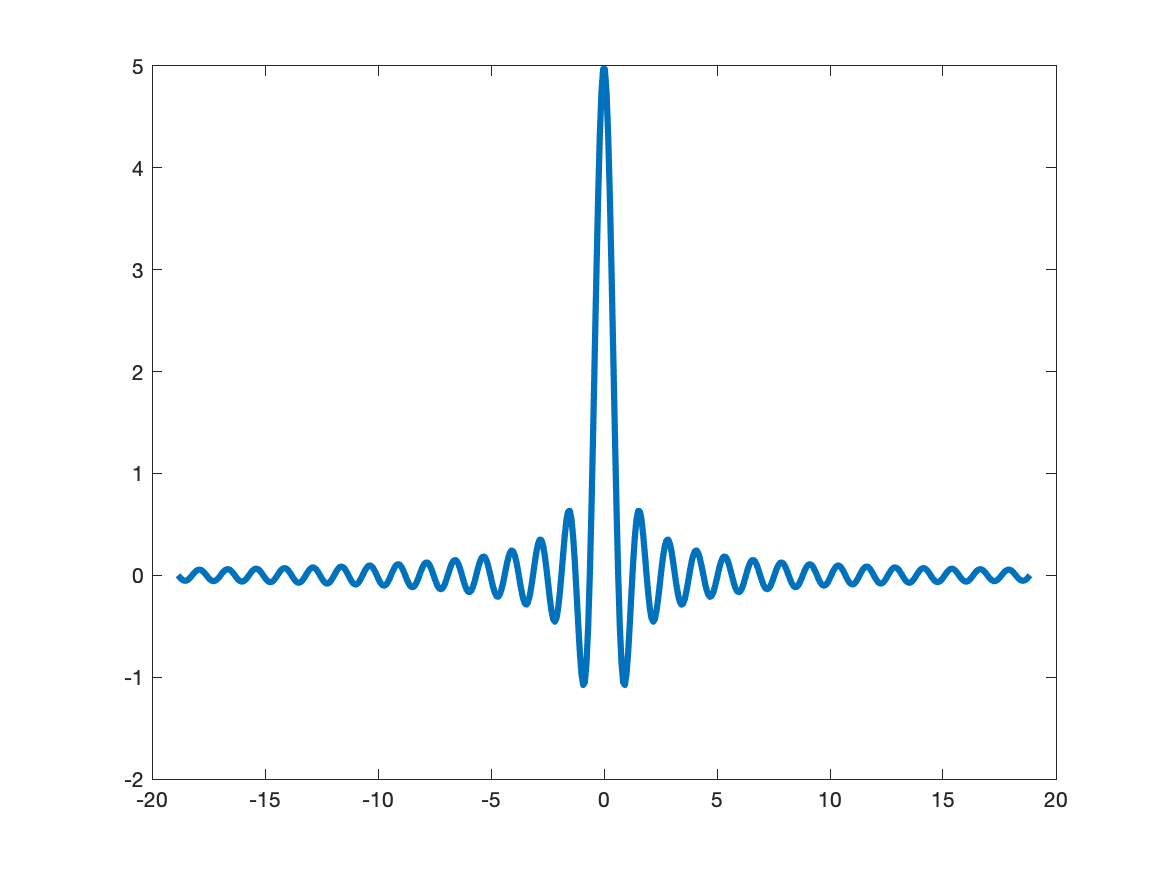
\includegraphics[width=5cm]{sincSignal1.png}
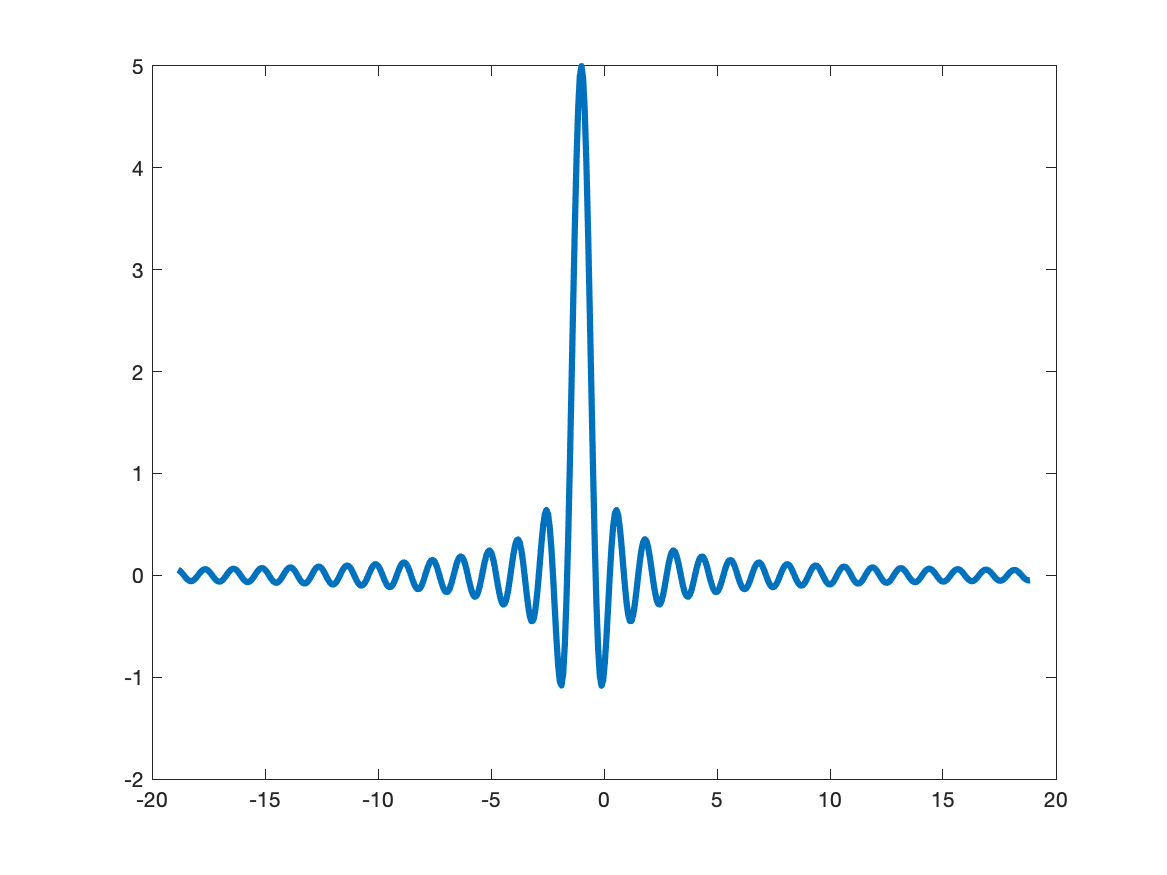
\includegraphics[width=5cm]{sincSignal2.png}
\end{center}

Measure is very sensitive to translation

\end{frame}

\begin{frame}
\frametitle{Measuring closeness - metrics }

Which of these images are closer
\begin{center}
\includegraphics[width=3cm]{whiteDog}
\includegraphics[width=3cm]{whiteCar}
\includegraphics[width=3cm]{blackDog}
\end{center}


\end{frame}

\begin{frame}
\frametitle{Measuring closeness - metrics }

Many different definitions of distance based on the application
\begin{itemize}
\item Normed distance
\item Hamming distance - for strings
\item Wasserstein metric - for probabilities (also applied to images)
\item Riemannian metrics - for data that "lives" on manifolds
\end{itemize}


\bigskip

Choosing the right distance is the key for the application

In many cases - chicken and egg. If we know the right distance then we know how to cluster.

\bigskip

We will use $L_2$ distance for conveniency.

\end{frame}

\begin{frame}
\frametitle{Using metrics - graphical models }

A graph is

A vertex set ${\cal V}$
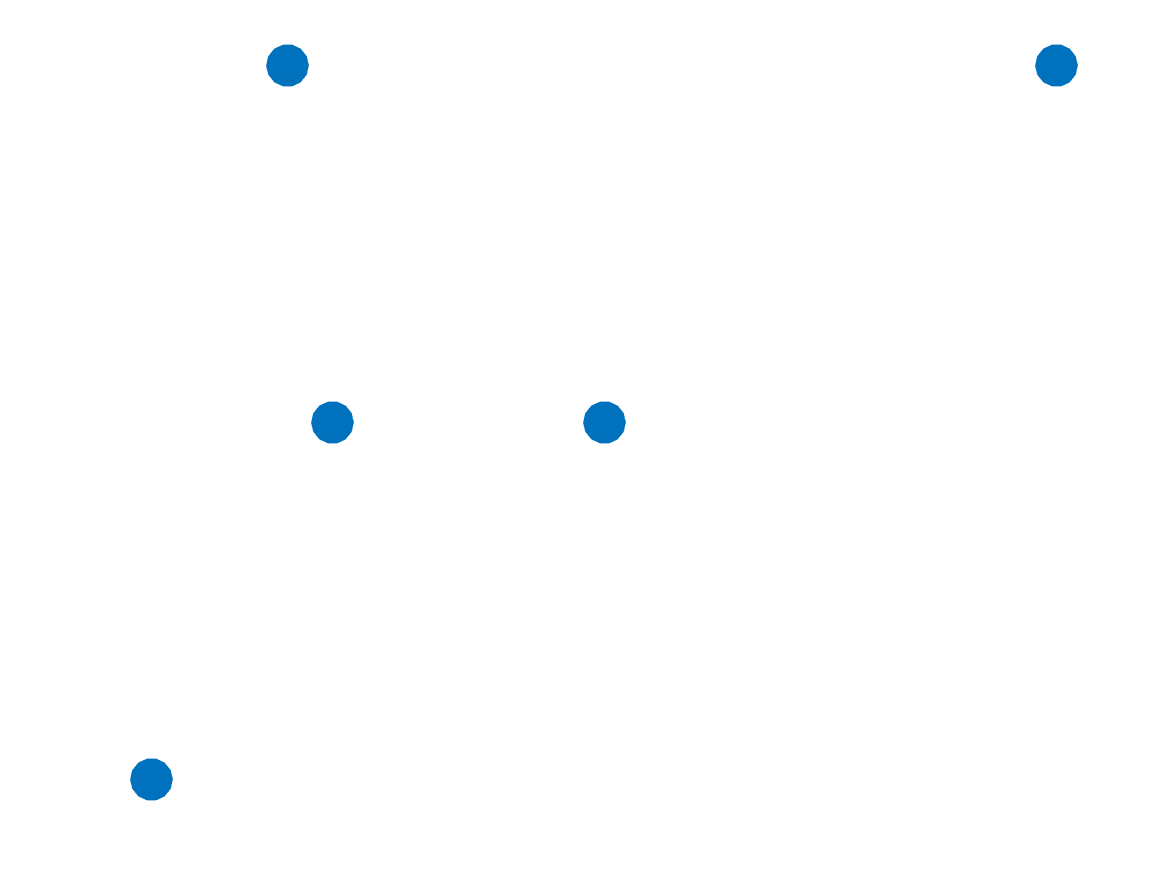
\includegraphics[width=3cm]{dots}

\pause

Edge set ${\cal E}$
\includegraphics[width=3cm]{dotsWithLines}


\end{frame}

\begin{frame}
\frametitle{The adjacency matrix }

The adjacency matrix is defined as
\begin{eqnarray*}
\bfA_{ij} = 	\left\{  \begin{matrix} 1 & {\rm if \ there\ is\ an \ edge} \\
						0 & {\rm otherwise}  \\
						0  & {\rm if }\ i=j \end{matrix} \right. 
\end{eqnarray*}

\includegraphics[width=5cm]{dotsWithLines}
$ \bfA = \begin{pmatrix} 0 & 1 & 1 & 1 & 1 \\
                                        1 & 0 & 1 & 1 & 0 \\
                                        1 & 1 & 0 & 1 & 1 \\
                                        1 & 1 & 1 & 0 & 1 \\
                                        1 & 0 & 1 & 1 & 0 \end{pmatrix} $



\end{frame}

\begin{frame}
\frametitle{The graph Laplacian }

The degree matrix
$$ {\bfD}   = {\rm diag}\left( \sum_j \bfA{ij} \right) $$ 

\includegraphics[width=5cm]{dotsWithLines}
$ \bfA = \begin{pmatrix} 0 & 1 & 1 & 1 & 1 \\
                                        1 & 0 & 1 & 1 & 0 \\
                                        1 & 1 & 0 & 1 & 1 \\
                                        1 & 1 & 1 & 0 & 1 \\
                                        1 & 0 & 1 & 1 & 0 \end{pmatrix}  \quad
   \bfD = \begin{pmatrix} 4 & 0 & 0 & 0 & 0 \\
                                        0 & 3 & 0 & 0 & 0 \\
                                        0 & 0 & 4 & 0 & 0 \\
                                        0 & 0 & 0 & 4 & 0 \\
                                        0 & 0 & 0 & 0 & 3 \end{pmatrix} 
                                        $


\end{frame}

\begin{frame}
\frametitle{The graph Laplacian }

The graph Laplacian
$$ {\bfL} = {\bfD}   - \bfA $$ 

$ \bfA = \begin{pmatrix} 0 & 1 & 1 & 1 & 1 \\
                                        1 & 0 & 1 & 1 & 0 \\
                                        1 & 1 & 0 & 1 & 1 \\
                                        1 & 1 & 1 & 0 & 1 \\
                                        1 & 0 & 1 & 1 & 0 \end{pmatrix}  \quad
   \bfD = \begin{pmatrix} 4 & 0 & 0 & 0 & 0 \\
                                        0 & 3 & 0 & 0 & 0 \\
                                        0 & 0 & 4 & 0 & 0 \\
                                        0 & 0 & 0 & 4 & 0 \\
                                        0 & 0 & 0 & 0 & 3 \end{pmatrix} 
                                        $

\bigskip

$ \bfL = \begin{pmatrix} 4 & -1 & -1 & -1 & -1 \\
                                        -1 & 3 & -1 & -1 & 0 \\
                                        -1 & -1 & 4 & -1 & -1 \\
                                        -1 & -1 & -1 & 4 & -1 \\
                                        -1 & 0 & -1 & -1 & 3 \end{pmatrix}  $

Note
$$ (\bfL \bfv)_i =  \sum_{i\not=j}  \bfv_i - \bfv_j \quad {\rm and} \quad \bfv^{\top}\bfL \bfv =  \sum_{e_{ij}}  (\bfv_i - \bfv_j)^2$$

\end{frame}

\begin{frame}
\frametitle{The weighted graph Laplacian }

In the Laplacian above every neighbour gets the same weight.

Define the weighted Laplacian, where each edge $e_{ij}$ is associated with a weight $0 \le w_{ij} $.
$$ (\bfL \bfv)_i =  \sum_{i\not=j}  \bfw_{ij}(\bfv_i - \bfv_j) \quad {\rm and} \quad \bfv^{\top}\bfL \bfv =  \sum_{e_{ij}} \bfw_{ij} (\bfv_i - \bfv_j)^2$$

Typical choice for $\bfw$ is
$$ \bfw_{ij} = \exp\left(-{\frac {\|\bfv_i - \bfv_j\|^2}{\sigma}} \right) $$

More appropriate choice
$$ \bfw_{ij} = \exp\left(-{\frac {D(\bfv_i,\bfv_j)}{\sigma}} \right) $$

\end{frame}

\begin{frame}
\frametitle{The eigenvalues and eigenvectors of the Laplacian }

The smallest eigenvalue is always $0$ with eigenvector $\bfv = [1,\ldots,1]^{\top}$ (why)


The second to smallest eigenvalue that is not zero is the Fiedler eigenvalue.

\centering
\includegraphics[width=5cm]{twoClasses.png}

It gets the (approximate) value $1$ on the first group and $-1$ (approximately) on the second group.

\end{frame}

\begin{frame}
\frametitle{The eigenvalues and eigenvectors of the Laplacian }


The second eigenvalue is the solution to the optimization problem
\begin{eqnarray*}
\min_{\bfu\not=\gamma\bfe} && \hf \bfu^{\top} \bfL \bfu \\
{\rm subject\ to} && \|\bfu \| = 1
\end{eqnarray*}

\bigskip

{\bf Interpretation} \\
Try to find the non-constant vector with the minimal energy 

The solution should be "smooth" on the graph

\end{frame}

\begin{frame}
\frametitle{The eigenvalues and eigenvectors of the Laplacian }


The second eigenvalue is the solution to the optimization problem
\begin{eqnarray*}
\min_{\bfu\not=\gamma\bfe} && \hf \bfu^{\top} \bfL \bfu \\
{\rm subject\ to} && \|\bfu \| = 1
\end{eqnarray*}


\bigskip

\begin{itemize}
\item
For small problems use eig solver of a dense matrix
\item
For large problem use iterative methods - inverse iteration, Krylov methods, randomized linear algebra
\end{itemize}

\bigskip

Power method
$$ \bfv_{k} = \bfL^{-\dag} \bfu_k \quad \quad \bfu_{k+1} = {\frac {\bfv_k}{\|\bfv_k\|}} $$


\end{frame}


\begin{frame}
\frametitle{The eigenvalues and eigenvectors of the Laplacian }

Example
\begin{center}
\begin{tabular}{ccc}
\includegraphics[width=3.5cm]{justDots.png} &
\includegraphics[width=3.5cm]{graphLap.png} &
\includegraphics[width=3.5cm]{fidlerVec.png} \\
Data & Graph Laplacian & Fidler Vector 
\end{tabular}
\end{center}

\end{frame}

\begin{frame}
\frametitle{The eigenvalues and eigenvectors of the Laplacian }

Can be very sensitive to parameters
\begin{itemize}
\item Number of neiboghrs
\item Choice of $\sigma$
\item Distance measure
\end{itemize}

\begin{center}
\begin{tabular}{ccc}
\includegraphics[width=3.5cm]{justDots3.png} &
\includegraphics[width=3.5cm]{graphLap3.png} &
\includegraphics[width=3.5cm]{fidlerVec3.png} \\
Data & Graph Laplacian & Fidler Vector 
\end{tabular}
\end{center}


\end{frame}

\begin{frame}
\frametitle{From unsupervised to semisupervised learning }

\begin{itemize}
\item
In most cases it is possible to obtain a few labeled data
\item 
Goal is to label the whole data given the labeled data
\item
Typically, results are much better and more robust than unsupervised learning
\end{itemize}

\bigskip

Assumption: we are given a set ${\cal S}$ where $\bfp_{{\cal S}}^{\rm obs}$ is the probability of each datum to belong to each class 


\end{frame}

\begin{frame}
\frametitle{From unsupervised to semisupervised learning }

{\bf Incorporating probabilities - the softmax function}

\begin{itemize}
\item $\bfp^{\rm obs}$ is a probability, $0 \le \bfp_i^{\rm obs} \le 1$ and $\sum \bfp^{\rm obs} = 1$.

\item $\bfu$ is unbounded 

\item Define $\bfp(\bfu) = {\frac {\exp(\bfu)}{\sum \exp(\bfu)}}$

\item Use cross entropy to compare probabilities, $\bfp(\bfu)$ and $\bfp^{\rm obs}$
$$ {\ell oss}(\bfu,\bfp^{\rm obs}) = -{\frac 1n} \bfp_{\rm obs}^{\top} \log(\bfp(\bfu)) $$

\end{itemize}

\end{frame}

\begin{frame}
\frametitle{From unsupervised to semisupervised learning }

{\bf New goal} - Fit the given labels {\bf and} keep the vector smooth.

$$ \min_{\bfu} \ {\cal E}(\bfu) = {\ell oss}(\bfu,\bfp^{\rm obs}) + {\frac \alpha 2} \bfu^{\top} \bfL \bfu $$ 

\begin{itemize}
\item $\alpha$ tradeoff parameter
\item Can be estimated using cross validation
\item Solution using inexact Newton's method
\end{itemize}

\end{frame}


\begin{frame}
\frametitle{From unsupervised to semisupervised learning }

{\bf Example - classifying nonlinear data}

\begin{center}
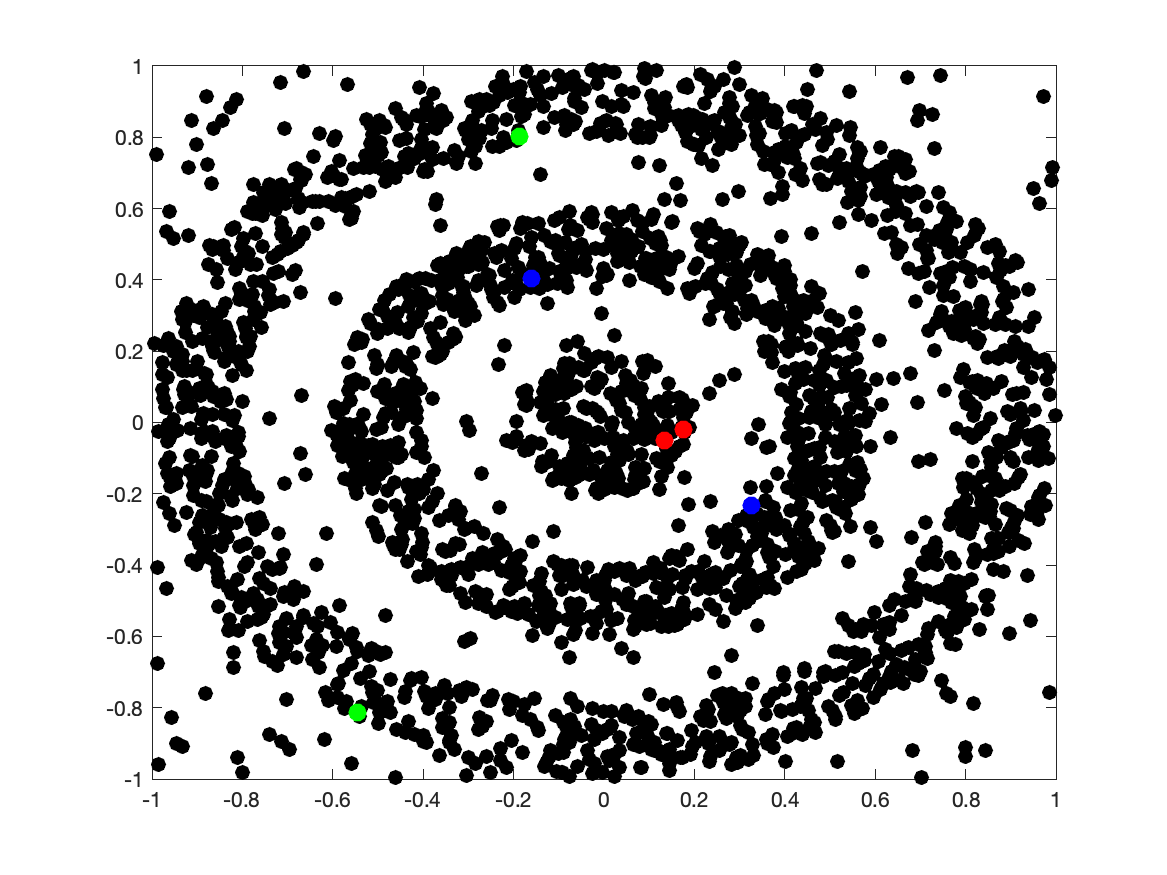
\includegraphics[width=5cm]{dataSemiSup.png} 
\begin{tabular}{cc}
\includegraphics[width=4.5cm]{graphLapCirc.png} &
\includegraphics[width=4.5cm]{graphLapCircReord.png} \\
Graph Lap &   Reordered Graph Lap 
\end{tabular}
\end{center}



\end{frame}

\begin{frame}
\frametitle{From unsupervised to semisupervised learning }


\begin{center}
\begin{tabular}{ccc}
\includegraphics[width=3.6cm]{probClass1.png} &
\includegraphics[width=3.6cm]{probClass2.png} &
\includegraphics[width=3.6cm]{probClass3.png} \\
Class 1 &  Class 2 & Class 3 
\end{tabular}
\end{center}


\end{frame}

\begin{frame}
\frametitle{Semisupervised learning - challenges}

\begin{itemize}
\item Choice of distance function
\item Choice of hyper parameters
\item Naive complexity $n^2$
\item Sparse linear algebra, preconditioning, eigenvalue solvers
\end{itemize}

\end{frame}


\end{document}

